%!TEX root = ../thesis.tex
\chapter{Preliminaries}
\label{preliminaries}

\section{Overview}
\label{preliminaries:overview}

Cryptography is the art and science of secure communication in the presence of third parties. As such, it has an immediate relationship with the privacy and anonymity requirement of data. Blockchain is a strong paradigm of cryptography embracement to enable the sought trust needed for exchanging digital assets. In this section we shall review the basic building blocks that cryptography provides to a data sharing system with the use of Blockchain. The purpose of the section is not about cryptography in itself but to merely lay the ground for the forthcoming chapters. As a result, the exposition style will not be formal in well know cases.

\section{Cryptographic Hash Functions}
\label{preliminaries:hash}

A hash function is a function that take an input of arbitrary length and returns a fixed-length value~\cite{crypto_101,boneh_crypto,kiagias:crypto,Katz:2014:IMC:2700550}. The output value is called digest.

Hash functions has many application. They are used in data structures such as hash tables, authentication schemes, password verification and data identifiers to name a few.

A hash function at minimum guarantees that for the same input yields the same output. Since the size of the output is fixed, the output range is finite. As a result, it is possible that for two different inputs a hash function produce the same output. This phenomenon is called collision.

Cryptographic hash functions have much stronger properties than regular hash function~\cite{crypto_101}. The ideal cryptographic hash function should be easily computable, noninvertible and collision-resistant~\cite{Katz:2014:IMC:2700550, kiagias:crypto}.

More formally, a cryptographic hash function $H$ is a deterministic polynomial algorithm that takes as input any string $x \in \{0, 1\}^{*}$ and outputs a string $H(x) \in \{0, 1\}^{k}$ where $k$ is of fixed size. A collision for a hash function $H$ is a pair of distinct messages $m_0, m_1$ where $m_0 \neq m_1$ and $H(m_0) = H(m_1)$. A hash function $H$ is collision-resistant if finding collisions is infeasible for any polynomial-time algorithm.

Typically there are three levels of security~\cite{Katz:2014:IMC:2700550}:

\begin{itemize}
  \item Preimage resistance: Given a digest $h$ it is hard to find any message $m$ with $H(m) = h$
  \item Second preimage resistance: For any given message $m_0$ it is hard to find a second message $m_1 \neq m_0$ such as $H(m_0) = H(m_1)$
  \item Collision resistance: It is hard to find a pair of messages $m_0, m_1$ where $m_0 \neq m_1$ and $H(m_0) = H(m_1)$
\end{itemize}

Above three, collision resistance is the strongest property and a strong security requirement.

In a data sharing system, cryptographic hash functions can be used to provide verification of file integrity and trackability~\cite{10.1109/SPW.2015.27, Azaria2016}. Anyone can detect file modification in transit as changing even a bit will result in the output of a different digest. A digest of a dataset or the dataset's metadata can also serve as means of unique file identification; unique persistent identifiers (PID) that can be used as pointers to data location. Any change to the PID will be visible and trackable~\cite{dist_pid}.

Blockchain make heavy use of cryptographic hash functions. They are used to create unique transactions and blocks IDs, to provide proof of inclusions--a proof that a transaction is contained in a block---and above all to prevent Sybil and double-spend attacks. It is evident, that cryptographic hash function play an important role in the Blockchain ecosystem.

\section{Symmetric-key cryptography}
\label{preliminaries:sym}

In a symmetric cryptosystem, two parties share a common secret key that has been agreed prior to communication. The key is used for both encryption and decryption. When a party wants to securely send a message uses the key to encrypt it and the receiver uses the same key to decrypt and recover the message. More formally, a symmetric cryptosystem is composed of the following algorithms~\cite{Katz:2014:IMC:2700550, kiagias:crypto}:

\begin{itemize}
  \item A key generation algorithm $\calg$ that takes as input a security parameter $1^{n}$ it and outputs a key $k$.
  \item An encryption algorithm $\cale$ that takes as input a key $k$ and a plaintext $m$ and outputs a ciphertext $c$.
  \item A decryption algorithm $\cald$ that takes as input a key $k$ and a ciphertext $c$ and outputs a plaintext $m$.
\end{itemize}

The set of all possible keys derived from the key generation algorithm $\calg$ is called the key space $\calk$. Respectively, the set of all possible plaintext is called the plaintext message space, denoted $\calm$, and the set of all possible ciphertexts is called ciphertext message space, denoted $\calc$. In practice keys are usually of some fixed length; 256-bit keys are very common. On the other hand, messages and ciphertexts can be of arbitrary length. For example, a message may be a video or a music file or even a single bit.

A symmetric cryptosystem must satisfy the correctness property: for all $m \in \calm$ and $k \in \calk$, it holds that

\begin{equation*}
  \cald_{k}(\cale_{k}(m)) = m
\end{equation*}

Any deterministic cryptosystem can not be secure~\cite{Katz:2014:IMC:2700550, kiagias:crypto}. To this end, randomness is essential to any encryption scheme.

In the following chapters, the notions of cipher and symmetric encryption scheme or symmetric scheme are identical and will be used interchangeably.

\subsection{One-time pad}
\label{preliminaries:sym:otp}

A one-time pad (OTP) is an symmetric encryption scheme where the keys, messages, and ciphertexts are of the same length and the key is never reused or repeated. The scheme is defined as follows~\cite{kiagias:crypto, boneh_crypto}:

\begin{itemize}
  \item Space: $\calm = \calc = \calk = \{0, 1\}^{n}$
  \item Encryption: $Enc_k(m) = k \xor m$
  \item Decryption: $Dec_k(c) = k \xor c$
\end{itemize}

The one-time pad is a \textbf{perfectly secure} scheme~\cite{kiagias:crypto, boneh_crypto}. The main drawback lies in the fact that the key must be at least the length of the original message. If a party wants to encrypt and sent 1GB video to another party, they must have already share a 1GB key. It is proven~\cite{shannon_otp} that perfect security (or perfect secrecy) can only be achieved when the key size is at least as long as the size of the message. As a consequence, perfect security schemes are impossible to use in practice.

\subsection{Stream Ciphers}
\label{preliminaries:sym:stream}

In~\ref{preliminaries:sym:otp} we saw that a symmetric scheme to be perfectly secure, keys and messages must have at least the same length. However, with weaker notion of security we can create symmetric encryption schemes where the size of the key $k$ is much shorter than the original message. Stream ciphers can encrypt or decrypt arbitrary long messages with small fixed length size keys. Instead of using a key of size $n$, a shorter seed $s$ of $l$-bits, where $l$ is much smaller than $n$, is used as the symmetric key. Then from the seed $s$ a $n$-bit key is derived and is used for encryption and decryption. The seed $s$ is expanded to $n$ by a deterministic polynomial algorithm $G$ that maps $l$-bit strings to $n$-bit strings. The algorithm $G$ is called \textbf{pseudorandom generator} (PRG) and the following condition must hold for any PRG~\cite{Katz:2014:IMC:2700550}:

\begin{itemize}
  \item Expansion: On input $s \in \{0, 1\}^{l}$ outputs $k \in \{0, 1\}^{n}$ where $\forall l, n > l$
  \item Pseudorandomness: Lets $\cald$ be a distribution over strings of length $n$. $\cald$ is indistinguishable from the uniform distribution over strings of length $n$. In other words, it is infeasible for any polynomial-time algorithm to tell whether it is given a string sampled according to $\cald$ or uniformly at random.
\end{itemize}

So, with the use of PRGs we can construct encryption schemes with short key sizes and long messages. A stream chipher is defined as follows:

\begin{itemize}
  \item The key generation algorithm $\calg$: Takes as input a security parameter $1^{n}$ and outputs a seed $s \in \{0, 1\}^{l}$ chosen uniformly at random.
  \item The encryption algorithm $\cale$: Takes as input a seed $s \in \{0, 1\}^{l}$ and a message $m \in \{0, 1\}^{n}$ and outputs the ciphertext $c = Enc_s(m) = G(s) \xor m$
  \item The decryption algorithm $\cald$: Takes as input a seed $s \in \{0, 1\}^{l}$ and a cipher $c \in \{0, 1\}^{n}$ and outputs the plaintext $m = Dec_s(c) = G(s) \xor c$
\end{itemize}

\subsection{Block Ciphers}
\label{preliminaries:sym:block}

\subsubsection{Modes of Operation}
\label{preliminaries:sym:modes}

\begin{itemize}
  \item ECB
  \item CBC
  \item CFB
  \item OFB
  \item CTR
\end{itemize}

\section{Public Key Cryptography}
\label{preliminaries:pub}

As we see in~\ref{preliminaries:sym} a secret key has to been agreed prior to communication. In 1976, Whitfield Diffie and Martin Hellman published a paper called New Directions in Cryptography~\cite{Diffie:2006:NDC:2263321.2269104} that changed the way of communication. They proposed a protocol that enables two parties, having no prior communication, to establish a secret key over an insecure channel in the presence of eavesdropping adversaries. The protocol uses two keys, one for encryption and one for decryption. The encryption key is called the public key and the decryption key is called the private key. Every party has a key pair consist of a public and a private key. The public key is made available for anyone that want to encrypt a message for the receiver; The receiver may post the public key online beforehand. When a party wants to send a message to another party she use the public key of the person of interest and encrypts the message using that key. The receiver of the message decrypts the ciphertext with the use of her private key. Only the rightful owner of the private key can decrypt a message that was encrypt with the corresponding public key. In an essence, a key pair is an identity and Blockchain technology smartly utilizes that to provide anonymity to the users of the system.

More formally, a public-key encryption scheme is composed of the following probabilistic, polynomial-time algorithms~\cite{Katz:2014:IMC:2700550, kiagias:crypto}:

\begin{itemize}
  \item The key generation algorithm $\calg$: Take as input a security parameter $1^{n}$ it and outputs a key pair ($p_k$, $s_k$).
  \item The encryption algorithm $\cale$: Take as input a public key $p_k$ and a plaintext $m$ and outputs a ciphertext $c$.
  \item The decryption algorithm $\cald$: Take as input a private key $s_k$ and a ciphertext $c$ and outputs a plaintext $m$.
\end{itemize}

Likewise, a public-key cryptosystem must satisfy the correctness property: for all $m \in \calm$ and $(p_k, s_k) \in \calk$, it holds that

\begin{equation*}
  \cald_{s_k}(\cale_{p_k}(m)) = m
\end{equation*}

\subsection{Diffie–Hellman key exchange}
\label{preliminaries:pub:dh}

The protocol works as follows~\cite{Katz:2014:IMC:2700550, kiagias:crypto}:

\begin{enumerate}
  \item Alice and Bob  with the use of a group generation algorithm $\calg$ agree on the description of a finite group $\G$ with input $1^{n}$. The common input for Alice and Bob is the tuple $(p, m, g)$ where $p$ is a large prime and $g$ is the generator of the finite group $\G$ of order $m$.
  \item Alice choose a random index $x_a \rselect{\Z_m}$ and computes $y_a \leftarrow{g^{x_a}}modp$. Alice sends $y_a$ to Bob.
  \item Bob choose a random index $x_b \rselect{\Z_m}$ and computes $y_b \leftarrow{g^{x_b}}modp$. Alice sends $y_b$ to Bob.
  \item Alice outputs $k = y_b^{x_a}modp = g^{{x_a}{x_b}}modp$
  \item Bob outputs $k = y_a^{x_b}modp = g^{{x_a}{x_b}}modp$
\end{enumerate}

The security of Diffie–Hellman key exchange is based on the difficulty of the discrete log problem (DLOG), which is the problem of computing $x$ given $g^{x}$ in a cyclic group $\G$. A passive adversary cannot compute the private key $k$ because she does not know $x_a$ or $x_b$. To find them she have to compute the discrete log which is assumed to be hard.

\begin{figure}[!hb]
  \centering
  \begin{tikzpicture}
    \matrix (m)[matrix of nodes, column  sep=2cm,row  sep=4mm, nodes={draw=none, anchor=center,text depth=0pt} ]{
    Alice & & Bob\\
    $x_a \rselect{\Z_m}$ & & $x_b \rselect{\Z_m}$ \\
    $y_a \leftarrow{g^{x_a}}modp$ & & $y_b \leftarrow{g^{x_b}}modp$ \\
     & $y_a$ & \\
     & $y_b$ & \\
     $k = y_b^{x_a}modp$ & & $k = y_a^{x_b}modp$ \\
    };

    \draw[shorten <=-1.5cm,shorten >=-1.5cm] (m-1-1.south east)--(m-1-1.south west);
    \draw[shorten <=-1.5cm,shorten >=-1.5cm] (m-1-3.south east)--(m-1-3.south west);
    \draw[shorten <=-1cm,shorten >=-1cm,-latex] (m-4-2.south west)--(m-4-2.south east);
    \draw[shorten <=-1cm,shorten >=-1cm,-latex] (m-5-2.south east)--(m-5-2.south west);

  \end{tikzpicture}
  \caption{Diffie–Hellman key exchange}
  \label{fig:crypto:dh}
\end{figure}

\subsection{The RSA Cryptosystem}
\label{preliminaries:pub:rsa}

The RSA cryptosystem~\cite{rsa} was developed in 1977 at MIT by Ron Rivest, Adi Shamer, and Leonard Adleman and is still the most widely used. It was the first public-key encryption scheme that could both encrypt and sign messages~\cite{kiagias:crypto}.

It works as follows~\cite{Katz:2014:IMC:2700550, kiagias:crypto}:

\begin{itemize}
  \item Key Generation:
    \begin{enumerate}
      \item Select randomly to large primes $p, q$ of length $n$ bits
      \item Compute $N = p*q$
      \item Calculate $\phi(N) = (p - 1)(q - 1)$
      \item Find $e$ such that $gcd(e, \phi(N)) = 1$
      \item Compute $d = e^{-1} mod\phi(N)$
      \item Public key is $(N, e)$ and private key is $(N, d)$
    \end{enumerate}
  \item Encryption: On input a public key $p_k = (N, e)$ and a message $m$ it computes the ciphertext $c$ as $ Enc_{p_k}(m) = m^{e}modN$
  \item Decryption: On input a private key $s_k = (N, d)$ and a ciphertext $c$ it computes the message $m$ as $ Dec_{s_k}(c) = c^{d}modN = m^{ed}modN = m$
\end{itemize}

If $p, q$ are known or obvious any interested party can compute $\phi(N)$ and therefore $d$. The RSA Cryptosystem is secure under the assumption that factorization of $N$ is believed to be hard.

The above mention protocol is not secure as the encryption function is deterministic and for the same input is produces the same output. As mention, a deterministic cryptosystem is not secure. One way to randomize the encryption function, is by appending random padding to message.

\subsection{The El Gamal Cryptosystem}
\label{preliminaries:pub:el_gamal}

The El Gamal Cryptosystem~\cite{el_gamal} is another popular and wide-used encryption scheme. It is based on the Diffie–Hellman key exchange and the security of the system is based on the hardness of discrete log problem. It works as follows~\cite{Katz:2014:IMC:2700550, kiagias:crypto}:

\begin{itemize}
  \item Key generation:
    \begin{enumerate}
        \item Run a group generation algorithm $\calg$ to produce the description of a finite group $\G$ with input $1^{n}$. The output is the tuple $(p, m, g)$ where $p$ is a large prime and $g$ is the generator of the finite group $\G$ of order $m$.
        \item Select randomly $x \rselect{\Z_m}$
        \item Calculate $h = g^{x}modp$
        \item The public key is $((p, m, g), h)$
        \item The secret key is $x$
    \end{enumerate}
  \item Encryption: Encrypts a message $m \in \G$
    \begin{enumerate}
      \item Choose randomly $r \rselect{\Z_m}$
      \item Compute $G = g^{r}modp$
      \item Compute $M = mh^{r}modp$
      \item Return $c = (G, M)$
    \end{enumerate}
  \item Decryption: Decrypts a ciphertext $c = (G, M)$
    \begin{enumerate}
      \item Compute $m = M / G^{x} modp$
      \item Return $m$
    \end{enumerate}
\end{itemize}

Another way to express the security of El Gamal scheme is under the decisional Diffie Hellman problem (DDH) which states that the tuples $(g^a, g^b, g^c)$ and $(g^a, g^b, g^{ab})$ are indistinguishable by a probabilistic polynomial-time (PPT) adversary.

\section{Digital signatures}
\label{preliminaries:sign}

A digital signature is a fundamental cryptographic primitive. It can be considered as the equivalent to a handwritten signature. It is a scheme from presenting the authenticity of digital messages or documents.

In a digital signature scheme, each party holds a unique key pair $(p_k, s_k)$. The signing key $s_k$ is used to uniquely sign a message $m$ and the verification key $p_k$ to verify the signature. Only someone with knowledge of $s_k$ can sign a message, but all parties having access to $p_k$ can verify a signature.

Digital signatures have the following important properties:

\begin{itemize}
  \item Authentication: The message was signed by a known sender
  \item Non-repudiation: The sender cannot deny having sent the message
  \item Integrity: The message was not altered in transit
\end{itemize}

Digital signatures are commonly used for software distribution and financial transactions and in cases where forgery detection is important. Blockchain is empowered with digital signatures to provide asset ownership; the rightful owner sign the transaction to prove possession of the asset.

More formally, a digital signature scheme is composed of the following probabilistic polynomial-time algorithms~\cite{Katz:2014:IMC:2700550,kiagias:crypto}:

\begin{itemize}
  \item The key generation algorithm $Gen$: Take as input a security parameter $1^{n}$ and outputs a key pair ($p_k$, $s_k$).
  \item A signing algorithm $Sign$: Take a signing key $s_k$ and a message $m$ and produce a digital signature $\sigma$ of $m$
  \item A deterministic verification algorithm $Verify$: Take a verification key $p_k$ and a signature $\sigma$. It outputs $b=1$ or $b=0$ ($true$ or $false$) to indicate if the signature is valid.
\end{itemize}

The primary goal of digital signatures is unforgeability; an adversary cannot create a new valid message-signature pair without the corresponding sign key.

\subsection{El Gamal Signature Scheme}
\label{preliminaries:sign:el_gamal}

The El Gamal Signature Scheme~\cite{el_gamal} is a digital signature scheme based on the difficulty of the discrete logarithm problem as in~\ref{preliminaries:pub:el_gamal}.

The scheme works as follows:

\begin{itemize}
  \item Key Generation:
    \begin{enumerate}
      \item Choose a cryptographic hash function $H$ where $H: \{0, 1\}^{*} \rightarrow \{0, 1\}^{n}$
      \item Choose a prime $p$ such as the DLOG problem is difficult
      \item Find a generator $g$ of the group $\Z^{*}_{p}$
      \item Choose randomly $x \rselect{\Z_q}$
      \item Compute $h = g^{x} modp$
      \item Return $(h, x)$ where $h$ is the public key and $x$ the private key
    \end{enumerate}
  \item Sign: Sign a message $m \in \{0, 1\}^{*}$ with a private key $x$
    \begin{enumerate}
      \item Choose randomly $k \rselect{\Z_q}$ such that $gcd(k, p − 1) = 1$
      \item Compute $r = g^{k}modp$
      \item Compute $s = k^{-1}(H(m) + xr) mod(p - 1)$
      \item Return the signature $(r, s)$
    \end{enumerate}
  \item Verify: Verify a signature $(r, s)$ of the message $m$ with a public key $h$
    \begin{enumerate}
      \item Verify that $r \in \Z_q$ and $s \in \Z_q$. Else ouput $0$.
      \item Compute $v = H(m)$
      \item If $v \stackrel{?}{=} (h^{r}r^{s}) modp$ then output $1$ else $0$.
    \end{enumerate}
\end{itemize}

\subsection{Digital Signature Algorithm (DSA)}
\label{preliminaries:sign:dsa}

The Digital Signature Algorithm (DSA)~\cite{dsa_nist} has been standardised by the National Institute of Standards and Technology (NIST). DSA is a variant of the El Gamal signature scheme. The main advantage of DSA over El Gamal Signature is the size of the signature. DSA produce signatures of size $320$-bit in comparison to El Gamal that needs at least signatures of size $2048$-bit to be secure given todays security standards~\cite{dsa}.

The algorithm work as follows~\cite{dsa}:

\begin{itemize}
  \item Key Generation:
    \begin{enumerate}
      \item Choose a cryptographic hash function $H$ where $H: \{0, 1\}^{*} \rightarrow \{0, 1\}^{n}$
      \item Choose a prime $q$ of size $n$
      \item Choose a prime $p$ such that $p - 1$ is a multiple of $q$ of size $l$. The size of $l$ must be a multiple of $64$ between $512$ and $1,024$
      \item Choose randomly $a \rselect{\Z_p}$
      \item Compute $g = a^{(p - 1)/q} mod p$
      \item Choose randomly $x \rselect{\Z_q}$
      \item Compute $h = g^{x} modp$
      \item Return $((p, q, g), h, x)$ where $(p, q, g)$ is the public parameters of the algorithm, $h$ is the public key and $x$ the private key.
    \end{enumerate}
  \item Sign: Sign a message $m \in \{0, 1\}^{*}$ with a private key $x$
    \begin{enumerate}
      \item Choose randomly $k \rselect{\Z_q}$
      \item Compute $r = (g^{k}modp)modq$
      \item Compute $s = k^{-1}(H(m) + xr) modq$
      \item Return the signature $(r, s)$
    \end{enumerate}
  \item Verify: Verify a signature $(r, s)$ of the message $m$ with a public key $h$
    \begin{enumerate}
      \item Verify that $r \in \Z_q$ and $s \in \Z_q$. Else ouput $0$.
      \item Calculate $w = s^{-1}modq$
      \item Calculate $u_1 = (H(m)w)modq$
      \item Calculate $u_2 = (rw)modq$
      \item Calculate $v = ((g^{u_1}h^{u_2})modp)modq$
      \item If $v \stackrel{?}{=} r$ then output $1$ else $0$.
    \end{enumerate}
\end{itemize}

\subsection{RSA signatures}
\label{preliminaries:sign:rsa}

As describes in~\ref{preliminaries:pub:rsa} the RSA cryptosystem can be used to sign messages. The RSA digital signature scheme works as follows~\cite{Katz:2014:IMC:2700550, kiagias:crypto}:

\begin{itemize}
  \item Key Generation:
    \begin{enumerate}
      \item Select randomly to large primes $p, q$ of length $n$ bits
      \item Compute $N = p*q$
      \item Calculate $\phi(N) = (p - 1)(q - 1)$
      \item Find $e$ such that $gcd(e, \phi(N)) = 1$
      \item Compute $d = e^{-1} mod\phi(N)$
      \item Verification key is $(N, e)$ and signing key is $(N, d)$
    \end{enumerate}
  \item Sign: On input a sign key $s_k = (N, d)$ and a message $m \in \Z^{*}_{N}$ it computes the signature $\sigma$ as $ Sign_{s_k}(m) = m^{d}modN$
  \item Verify: On input a verification key $p_k = (N, e)$, a message $m \in \Z^{*}_{N}$ and a signature $\sigma \in \Z^{*}_{N}$ it outputs $1$ if and only if $m \stackrel{?}{=} Verify_{p_k}(\sigma, m) = \sigma^{e}modN$
\end{itemize}

The above signature scheme is not secure as an adversary can forge a sign, based on the public key alone, by choosing an arbitrary $\sigma \in \Z^{*}_{N}$ and compute $m = \sigma^{e}modN$. Another attack on the RSA signature scheme allows the adversary to output a forgery on any message of the adversary's choice. One proposal to protect against those attacks, that can be proven secure under certain assumptions, is by applying a cryptographic hash function $H$ to the message before sign it. The minimal requirement for the system to be secure is that $H$ must be collision-resistant.

\section{Elliptic-curves}
\label{preliminaries:el_curves}

Elliptic curves (ECC) play an import role in cryptography. All cryptosystems, defined in previous chaptes, are built over multiplicative groups of integers modulo a sufficient large prime $p$~\cite{kiagias:crypto, boneh_crypto}. Elliptic curves are additive abelian groups~\cite{kiagias:crypto}; a group satisfying associativity, commutativity, existence of identity element and inverse under the addition group operation~\cite{elliptic_curves_2}.

There are two apparent benefits for using curves over modular groups~\cite{kiagias:crypto}. The first is cost efficiency. In practice, cryptosystems that their security depends on the discrete log problem or the factorisation problem on a modular group, such as the El Gamal or the RSA, the primes have to be at least 2048 bits for the system to be secure. On the other hand, elliptic curves offer similar security using much smaller key sizes. A 233-bit elliptic curve key gives the same level of security as a 2,240-bit RSA key~\cite{ecc_rsa_bits, ecc_rsa_bits_1} and a 333-bit elliptic curve key as a 4096-bit RSA key~\cite{blake1999elliptic}. The second reason is that, for the moment, there is no know way to generalise the attacks against the discrete logarithm problem on a modular group to an attack on an elliptic curve~\cite{kiagias:crypto}.

Cryptography is primarily interested in elliptic curves over $\F_p$: the field of integers modulo $p$ where $p$ is a prime number. An elliptic curve $E$ over $\F_p$ is defined by the equation of the form~\cite{elliptic_curves, elliptic_curves_2}:

\begin{equation*}
  y^2 = x^3 + ax + b
\end{equation*}

where $a, b \in \F_p$. A pair $(x, y)$ where $x, y \in \F_p$ is a point on the curve if it satisfies the equation where $E$ is defined. There is a special point, called \textbf{point at infinity} and denoted by $\infty$, where is also on the curve and serve as the identity element~\cite{elliptic_curves_2}.

Let $P = (x_1, y_1)$ and $Q = (x_2, y_2)$ two points on the elliptic curve $E$. Any two points on a curve add to produce a third point on the curve. A third point $R$ on the curve $E$ is defined as~\cite{elliptic_curves}:

\begin{equation*}
  R = P + Q
\end{equation*}

We can find the third point $R$ as follows~\cite{elliptic_curves}:

\begin{enumerate}
  \item Draw the line $L$ through $P$ and $Q$
  \item $L$ intersects to a third point $-R$
  \item Reflect $-R$ across the $x$-axis to obtain $R$
\end{enumerate}

\begin{figure}
  \centering
  \begin{tikzpicture}
    \begin{axis}[
            xmin=-4,
            xmax=5,
            ymin=-5,
            ymax=5,
            xlabel={$x$},
            ylabel={$y$},
            scale only axis,
            axis lines=middle,
            domain=-1.3247:2,
            y domain=-3:3,
            samples=200,
            smooth,
            clip=false,
            axis equal image=false,
            ticks=none
        ]

    \addplot[red] {sqrt(x^3-x+1)} node[right, black] {$y^2 = x^3 -x + 1$};
    \addplot[red] {-sqrt(x^3-x+1)};

    \end{axis}
    \end{tikzpicture}
  \caption{Elliptic curve}
\end{figure}

\begin{figure}
  \centering
  \begin{tikzpicture}
    \begin{axis}[
            xmin=-4,
            xmax=5,
            ymin=-5,
            ymax=5,
            xlabel={$x$},
            ylabel={$y$},
            scale only axis,
            axis lines=middle,
            domain=-1.3247:2,
            y domain=-3:3,
            samples=200,
            smooth,
            clip=false,
            axis equal image=false,
            ticks=none,
        ]

    \addplot[red] {sqrt(x^3-x+1)} node[right, black] {};
    \addplot[red] {-sqrt(x^3-x+1)};
    \addplot[blue, domain=-3:3,] {0.27*x + 0.87};

    \draw [fill=black] (axis cs:-1.25, 0.535) circle (2pt);
    \draw [fill=black] (axis cs:0.165, 0.9) circle (2pt);
    \draw [fill=black] (axis cs:1.165, 1.17) circle (2pt);
    \draw [fill=black] (axis cs:1.165, -1.17) circle (2pt);

    \draw [dashed] (axis cs:1.165, 1.17) -- (axis cs:1.165,-1.17);

    \draw[color=black] (axis cs:-1.4, 0.635) node [left]{$P$};
    \draw[color=black] (axis cs:0.0, 1.5) node [left]{$Q$};
    \draw[color=black] (axis cs: 1.4, 1.6) node [left]{$-R$};
    \draw[color=black] (axis cs: 3.7, -1) node [left]{$R = P + Q$};

    \end{axis}
    \end{tikzpicture}
  \caption{Elliptic curve point addition}
\end{figure}

Cyclic subgroups of such elliptic curve groups can be used to implement discrete logarithm systems. The parameters that describe an elliptic curve $E$ defined over a finite field $\F_p$, a base (generator) point $P \in E$, and its order $q$ should be chosen carefully so that the elliptic curve discrete logarithm problem (ECDLP) is resistant to all known attacks. ECDLP is the problem of finding $d$ given $Q = dP$ and $P$ and is assumed to be hard.

Blockchain uses only elliptic curves for key pair generation and transaction signing (ECDSA). Bitcoin and Ethereum use a specific elliptic curve for ECDSA which is defined in the secp256k1 standard established by the National Institute of Standards and Technology (NIST).

\subsection[Key generation]{Key generation~\cite{elliptic_curves_2}}
\label{preliminaries:el_curves:key_gen}

Let $E$ be an elliptic curve over $\F_p$ and $P$ a generator point in $E$ of order $q$. The key pair generation algorithm is defined as follows:

\begin{enumerate}
  \item Select a random integer $d \rselect{\in \Z_q}$
  \item Compute $Q = dP$
  \item Return the tuple $(Q, d)$ where $Q$ is the public key and $d$ the secret key
\end{enumerate}

The prime $p$, the curve $E$ the generator point $P$, its order $q$ and the public key $Q$ are public and finding the secret key $d$ is equivalent to solving the ECDLP.

\subsection{Diffie-Hellman key exchange}
\label{preliminaries:el_curves:dh}

The elliptic curve analogue of Diffie-Hellman key exchange protocol (ECDH) defined in~\ref{preliminaries:pub:dh} can implemented as follows~\cite{elliptic_curves}:

\begin{enumerate}
  \item Alice and Bob agree on elliptic curve $E$ over a finite field $F_p$ for a prime $p$ such that the discrete log problem is hard in $E$ over $F_p$. They also agree on a point $P$ on $E$.
  \item Alice choose a secret integer $a$ and computes $P_a = aP$. Alice sends $P_a$ to Bob
  \item Bob choose a secret integer $b$ and computes $P_b = bP$. Bob sends $P_b$ to Alice
  \item Alice computes $k = aP_b = abP$
  \item Bob computes $k = bP_a = abP$
\end{enumerate}

The security of the protocol is based on ECDLP (§~\ref{preliminaries:el_curves:key_gen}).

\subsection{The El Gamal Cryptosystem}
\label{preliminaries:el_curves:el_gamal}

The elliptic curve analogue of El Gamal cryptosystem defined in~\ref{preliminaries:pub:el_gamal} can implemented as follows~\cite{elliptic_curves_2}:

\begin{itemize}
  \item Key generation: Run elliptic curve key generation algorithm defined in~\ref{preliminaries:el_curves:key_gen} and get a key pair $(Q, d)$.
  \item Encryption: Encrypts a message $m$ represented as a point $M$ in $E$ over $\F_p$
    \begin{enumerate}
      \item Choose randomly $r \rselect{\in \Z_q}$
      \item Compute $G = rP$
      \item Compute $C = M + rQ$
      \item Return $c = (G, C)$
    \end{enumerate}
  \item Decryption: Decrypts a ciphertext $c$
    \begin{enumerate}
      \item Compute $M = C - dG$, and extract $m$ from $M$
      \item return $M$
    \end{enumerate}
\end{itemize}

An eavesdropper adversary who wants to obtain $M$ needs to compute $rQ$; given $Q$, $P$ and $G = rP$ find $r \in Z_q$. This is the elliptic curve analogue of the Diffie-Hellman problem.

\subsection{Elliptic Curve Digital Signature Algorithm (ECDSA)}
\label{preliminaries:sign:el_curves:ecdsa}

The Elliptic Curve Digital Signature Algorithm (ECDSA) is a variant of the Digital Signature Algorithm (DSA) which use elliptic Curves. It is the most widely standardised elliptic curve-based signature scheme~\cite{elliptic_curves_2}.

Let $E$ be an elliptic curve over $\F_p$, a generator point $P$ of order $q$ and $H$ a cryptographic hash function where $H: \{0, 1\}^{*} \rightarrow  \{0, 1\}^{q}$. The ECDSA is defined as follows~\cite{elliptic_curves_2}:

\begin{itemize}
  \item Key generation: Run elliptic curve key generation algorithm defined in~\ref{preliminaries:el_curves:key_gen} and get a key pair $(Q, d)$.
  \item Sign: Sign a message $m$ with a private key $d$
    \begin{enumerate}
      \item Choose randomly $k \rselect{\Z_q}$
      \item Compute the point $kP = (x_1, y_1)$
      \item Compute $r = x_1modq$. If $r \stackrel{?}{=} 0$ then go to step 1
      \item Compute $e = H(m)$
      \item Compute $s = k^{-1} (e + dr) modq$. If $s \stackrel{?}{=} 0$ then go to step 1
      \item Return the signature $(r, s)$
    \end{enumerate}
  \item Verify: Verifies a signature $(r, s)$ of the message $m$ with a public key $Q$
    \begin{enumerate}
      \item Verify that $r \in \Z_q$ and $s \in \Z_q$. Else ouput $0$.
      \item Compute $e = H(m)$
      \item Compute $w = s^{-1}modq$
      \item Compute $u_1 = (ew)modq$ and $u_2 = (rw)modq$
      \item Compute $X = u_1P + u_2Q$
      \item If $X \stackrel{?}{=} \infty$ output $0$
      \item Take $x_1$ cordinate of $X$ and compute $v = x_1modq$
      \item If $v \stackrel{?}{=} r$ then output $1$ else $0$.
    \end{enumerate}
\end{itemize}

\section{Homomorphic Encryption}
\label{preliminaries:homo}

Homomorphic encryption allows computation on encrypted data. It allows, without having access to unencrypted data, to perform computations over ciphertexts and return encrypted results that when decrypted matches the result of the operations as if they had been performed on the plaintext.

\begin{equation*}
  Enc(m_1) \otimes Enc(m_2) = Enc(m_1 \oplus m_2)
\end{equation*}

\section{Zero Knowledge Proofs}
\label{zkp}

A proof of knowledge is a protocol that enables one party to convince another of the validity of a statement.
In a zero-knowledge proof, this is accomplished without revealing any information beyond the legitimacy of the proof~\cite{kiagias:crypto},
meaning that one party can prove to another party that a given statemnet is true, without conveying any information apart from
the fact that the statement is indeed true~\cite{wiki:zkp}.

Let $\calp$ be a prover and $\calv$ the verifier. $\calp$ must convince $\calv$ that she has some
knowledge of a statement $x$ without explicitly stating what she knows. We call this knowledge a witness $w$.
Both parties are aware of a predicate $R$ that will attest to $w$ being a valid witness to $x$~\cite{kiagias:crypto}. In general,

\begin{itemize}
  \item The predicate $R$ is assumed to be polynomial-time computable.
  \item The prover $\calp$ has $R,x$, and $w$ such that $R(x,w) = 1$. She wishes to prove possesion of $w$ by producing a proof of knowledge $\pi$.
  \item The verifier $\calv$ has $R,x$, and $\pi$.
  \item Given $R$ it is hard to find a corresponding $w$ such as $R(x,w) = 1$
  \item The prover $\calp$ is reluctant to reveal $w$; otherwise the solution is trivial.
  \item The verifier $\calv$ can efficiently check the validity of $\pi$.
\end{itemize}

\subsection{Examples}

\subsubsection{The strange cave of Ali Baba}
\label{zkp:examples}

Suppose there is our old friends Alice and Bob. At the bottom of the cave~\cite{Quisquater:1989:EZP:118209.118269} of figure~\ref{fig:zkp:alibaba} there is a magic door that
can only be open using a secret password. The cave is shaped like a rentacle with one entrace at one side and the magic door blocking the opposite side.
Bob knows the secret password and wants to prove to Alice that he can open the magic door without revealing the password to Alice.
Bob propose the following game to prove to Alice he can open the magic door: Alice waits outside the cave, Bob enters the cave and
takes either left or right path. Alice can not see which path Bob takes. Then Alice enters, stants at the entrance of cave and calls
Bob to come out either the left or the right passage. Bob complies, using the secret password if necessary.

If Bob does not know the secret password he has $1/2$ change of guessing correctly (he would only be able to return by the named path if
Alice were to give the name of the same path by which he had entered) as Alice choose at random which path Bob should take. If they repeat this procedure
$k$ times the probability of Bob convincing Alice that he knows the secret password without actually knowing it reduce exponetially. In particular, at most $1/2^{k}$.

\subsubsection{The colour-blind friend}

Let's bring again our friends Alice and Bob. Suppose Bob is color-blind~\cite{wiki:zkp,zkp:colour_blind} and Alice has two balls: one red and one green but otherwise identical when you touch them.
To Alice they seem complete identical and she is not sure if they are actually distinguishable. Bob wants to prove to Alice that indeed the are differently-coloured
without revealing which one is red and which is green. To prove his knowledge, Bob gives to Alice the two balls so that she is holding one in each hand. Bob can see
at this point which ball is in which hand. Next, Alice either switches the ball behind her hands or leaves them be, with probability $1/2$. Finally, she brings
them out from behind her back. Alice then asks Bob if she switch the balls. By looking at their colors, Bob can can say with certainty whether he switched them or not.
On the other hand, if they were the same color and hence indistinguishable, there is no way you could guess correctly with probability higher than 1/2. If they repeat
this procedure $k$ times the probability that Bob succeeded at identifying all the switch/non-switches when the balls are identical (thus lying to Alice) is at most
$1/2^{k}$.

\begin{figure}[t!]
  \centering
  \begin{subfigure}[t]{0.30\textwidth}
    \centering
    \resizebox{\linewidth}{!}{
      \begin{tikzpicture}[scale=1]
        % Cave %
        \draw(0,5) -- (2,5) -- (2,8) -- (10,8) -- (10,4);
        \draw(0,4) --(2,4) -- (2,1) -- (10,1) -- (10, 4);
        \draw(9,4.5) -- (10,4.5);
        \draw(3,5) -- (3,7) -- (9,7) -- (9,5);
        \draw(3,5) -- (3,2) -- (9,2) -- (9,5);
        % Actors %
        \draw[fill] (1,5.6) circle [radius=0.1];
        \node [below] (alice) at (1,5.5) {Alice};
        \draw[fill] (2.5,4.6) circle [radius=0.1];
        \node [below] (bob) at (2.5,4.5) {Bob};
        % Arrows %
        \draw [dashed, ->] (2.5,4.6) -- (2.5,6);
        \draw [dashed, ->] (2.5,3.9) -- (2.5,2);

      \end{tikzpicture}
    }
    \caption{Alice stands outside and Bob choose randomly a path, left or right}
    \label{fig:zkp:alibaba:a}
  \end{subfigure}
  \begin{subfigure}[t]{0.30\textwidth}
    \centering
    \resizebox{\linewidth}{!}{
      \begin{tikzpicture}[scale=1]
        % Cave %
        \draw(0,5) -- (2,5) -- (2,8) -- (10,8) -- (10,4);
        \draw(0,4) --(2,4) -- (2,1) -- (10,1) -- (10, 4);
        \draw(9,4.5) -- (10,4.5);
        \draw(3,5) -- (3,7) -- (9,7) -- (9,5);
        \draw(3,5) -- (3,2) -- (9,2) -- (9,5);
        % Actors %
        \draw[fill] (2.5,4.6) circle [radius=0.1];
        \node [below] (alice) at (2.5,4.5) {Alice};
        \draw[fill] (9.5,4.3) circle [radius=0.1];
        \node [below] (bob) at (9.5,4.2) {Bob};
        % Speech Bubble %
        \node[overlay,draw,cloud callout,callout relative pointer={(0.2cm,-0.7cm)},%
        aspect=2.5,fill=white!90] at ($(alice)+(-0.5cm,2.3cm)$) {Left};

      \end{tikzpicture}
    }
    \caption{Alice calls to Bob, asking him to come out either the left or the right passage}
    \label{fig:zkp:alibaba:b}
  \end{subfigure}
  \begin{subfigure}[t]{0.30\textwidth}
    \centering
    \resizebox{\linewidth}{!}{
      \begin{tikzpicture}[scale=1]
        % Cave %
        \draw(0,5) -- (2,5) -- (2,8) -- (10,8) -- (10,4);
        \draw(0,4) --(2,4) -- (2,1) -- (10,1) -- (10, 4);
        \draw(9,4.5) -- (9.5,4.5);
        \draw(3,5) -- (3,7) -- (9,7) -- (9,5);
        \draw(3,5) -- (3,2) -- (9,2) -- (9,5);
        % Actors %
        \draw[fill] (2.5,4.6) circle [radius=0.1];
        \node [below] (alice) at (2.5,4.5) {Alice};
        \draw[fill] (2.5,7.8) circle [radius=0.1];
        \node [below] (bob) at (2.5,7.7) {Bob};
        % Speech Bubble %
        \node[overlay,draw,cloud callout,callout relative pointer={(0.2cm,-0.7cm)},%
        aspect=2.5,fill=white!90] at ($(alice)+(-0.5cm,2.3cm)$) {OK};

      \end{tikzpicture}
    }
    \caption{Bob complies appearing at the exit Alices names}
    \label{fig:zkp:alibaba:c}
  \end{subfigure}
  \caption{Ali Baba Cave}
  \label{fig:zkp:alibaba}
\end{figure}

\subsection{Formal Definition}
\label{zkp:definition}

Let $<\calp, \calv>$ be a pair of interactive programs. Define $\text{out}^{\calp}_{\calp, \calv}(x,w,z)$
to be the output of $\calp$ when both $\calp$ and $\calv$ are executed with the public input $x$ and private
inputs $w$ and $z$ ($\calp$ determines $w$ and $\calv$ choose $z$); $\text{out}^{\calv}_{\calp, \calv}(x,w,z)$
is similar defined for $\calv$. The PPT interactive protocol $<\calp, \calv>$ is a \textbf{zero-knowledge proof}
for a language $L \in NP$ with knowledge error $k$ and zero-knowledge distance $\e$ if the following
properties hold~\cite{kiagias:crypto}.

\begin{enumerate}
  \item \textbf{Completeness:} If $x \in L$ and $R(x,w) = 1$ for some witness $w$, then $\text{out}^{\calv}_{\calp, \calv}(x,w,z)$ = 1
    for all string $z$ with overwhelming probability in $v$.
  \item \textbf{Soundness:} For any polynomial-time program $\calp^{*}$ define for arbitrary $x,w,z,$
    \begin{equation*}
      \pi_{x,w,z} = \Prob[\text{out}^{\calv}_{\calp^{*}, \calv}(x,w,z) = 1].
    \end{equation*}
    A protocol $<\calp, \calv>$ satisfies soundness if there are non-negligible functions $s(v), q(v)$ such for all $\calp^{*}$ here exists a probabilistic
    Turing machine (PTM) program $K$, called a knowledge extractor with the following property. Suppose that

    \begin{equation*}
      \widetilde{\pi} = \Prob[K(x,w,z) = w^{'} : R(x, x^{'}) = 1].
    \end{equation*}
    Then it holds that $\pi_{x,w,z} \geq s(|x|)$ implies that $\widetilde{\pi}_{x,w,z} \geq q(\abs{x})$.

  \item \textbf{(Statistical) Zero-knowledge:} For each polynomial-time program $\calv^{*}$, there is a PTM program $S$, called the \textbf{simulator}, such that for all
    $x,w$ with $R(x,w) = 1$, the random variables $S(x,z)$ and $\text{out}^{\calv^{*}}_{\calp, \calv^{*}}(x,w,z)$ are statistically indistinguishable for all strings $z$:
    \begin{equation*}
      \forall \cala \abs[\Big]{\Prob[\cala(S(x,z) = 1)] - \Prob[\cala(\text{out}^{\calv^{*}}_{\calp, \calv^{*}}(x,w,z)) = 1]} < \e.
    \end{equation*}
\end{enumerate}

Completeness is very similar to correctness. Assuming both the prover and verifier follow the protocol faithfully, completeness guarantees that the
protocol will succeed with a sufficiently high probability.
Soundness ensures that if the statement is false, no cheating prover can convince the honest verifier that it is true, except with some small probability.
Intuitively, statistical zero-knowledge is a property that prohibits a verifier from extracting information from an honest prover.
A weaker version of zero-knowledge is honest-verifier zero-knowledge (HVZK). Here it is assumed that the verifier executes the protocol faithfully,
but makes additional computations~\cite{kiagias:crypto}.

\subsection{zk-SNARKs}
\label{zkp:snarks}

Since computational power is often limited to devices such as mobiles or IoT (clients) the need of outsourcing computation to one or more powerful workers on the cloud emerges. Yet, confidence is needed at the working entity for proper computation. For this reason, the client should be able to verify the correctness of the results returned. That way not only the client is protected from malicious or malfunctioning workers but also the legitimate worker is benefit by shedding liability~\cite{pinocchio-nearly-practical-verifiable-computation}. This scheme is called public verifiable computation (VC).

In a public verifiable computation scheme the client outsource the evaluation of a function $F$ on input $u$ known to the client (e.g. a query). The client then can verify the correctness of the computation of $F(u)$ with less work than required for the computation of $F(u)$. When the outsource function $F$ consist of two inputs $u$ and $w$, where $w$ is the worker's private input (e.g a data set), then the scheme is a Zero-Knowledge Verifiable Computation (or non-interactive zero knowledge (NIZK) proof~\cite{Blum:1991:NZ:123137.123145}) if the client learns nothing about worker's input expect the output of the computation~\cite{pinocchio-nearly-practical-verifiable-computation}.

Such schemes are not interactive meaning no interaction is necessary between prover and verifier (worker and client) and a common reference string (CRS) shared between them is enough to achieve computational zero-knowledge~\cite{Blum:1991:NZ:123137.123145}.

Formally, as defined by Parno et. al~\cite{pinocchio-nearly-practical-verifiable-computation} a public Zero-Knowledge verifiable computation scheme $\calv \calc$ consist of a set of three polynomial-time algorithms:

\begin{itemize}
  \item $(EK_F, VK_F) \leftarrow \text{KeyGen}(F, 1^{\lambda})$: The randomized key generation algorithm. It takes as input the outsourced function $F$ and a security parameter ${\lambda}$; it outputs a public evaluation key $EK_F$ and a public verification key $VK_F$.
  \item $(y, \pi_y) \leftarrow \text{Compute}(EK_F, u)$: The deterministic worker algorithm. It takes as input the public evaluation key $EK_F$ and a public input $u$; it outputs $y \leftarrow F(u, w)$, where $w$ is an auxiliary private input, and a proof $\pi$ of $y$'s correctness.
  \item $\{0, 1\} \leftarrow \text{Verify}(VK_F, u, y, \pi_y)$:  The deterministic verification algorithm. It takes as input the public verification key $VK_F$, the public input $u$, the output $y$ and the proof $\pi_y$; It outputs $1$ if $F(u) = y$ and $0$ otherwise.
\end{itemize}

The acronym zk-SNARK stands for `Zero-Knowledge Succinct Non-Interactive Argument of Knowledge` in which each individual part, informally, have the following meaning~\cite{zksnarks_nutshell, zcash, 184425, Bitansky:2012:ECR:2090236.2090263}:

\begin{itemize}
  \item Zero-Knowledge: The verifier learns nothing but the validity of the computation
  \item Succinct: The proof are sort and easy to verify in comparison to the actual computation (constant size and polynomial verifiable in the size of the proof)
  \item Non-Interactive: There is no or little interaction done in one step. Anyone can verify without the need of interacting anew (publicly verifiable)
  \item ARgument: Soundness (§~\ref{zkp:definition}) holds only against computationally bounded provers
  \item of Knowledge: If the verifier accepts a proof output by a computationally bounded prover, then the prover has a witness for the given instance
\end{itemize}

At high level, zkSNARKs consist of four basic steps (Figure ~\ref{fig:zkp:zksnark_flow}):

\begin{enumerate}
  \item Computation to Arithmetic circuit~\cite{wiki:circuits}
  \item Arithmetic circuit to Rank 1 Constraint System (R1CS)~\cite{ggpr}
  \item R1CS to Quadratic Span Program (QAP)~\cite{ggpr}
  \item QAP to zkSNARK~\cite{pinocchio-nearly-practical-verifiable-computation}
\end{enumerate}

The main idea for constructing zkSNARKs is firstly to transform the generic program as a quadratic equation of polynomials (QAP)~\cite{ggpr}: $p(x)q(x) = s(x)r(x)$, where the equality holds if and only if the program is computed correctly. So the prover wants to convince the verifier that the equality holds.

Succinctness is achieved by random sampling. The verifier chooses a secret evaluation point $x_0$ to reduce the problem from polynomial multiplication and equality to simple number arithmetic checks: $p(x_0)q(x_0) = s(x_0)r(x_0)$. To allow the prover to compute the evaluation of the polynomials at $x_0$, without revealing $x_0$, Homomorphic encryption is used:  $E(p(x_0))E(q(x_0)) = E(s(x_0))E(r(x_0))$

Finally the prover obfuscates the encrypted values by multiplying with a number so that the verifier can still check the correctness of the structure without knowing the actual
encrypted values: $E(k + p(x_0))E(k + q(x_0)) = E(k + s(x_0))E(k + r(x_0))$

\begin{figure}[ht!]
  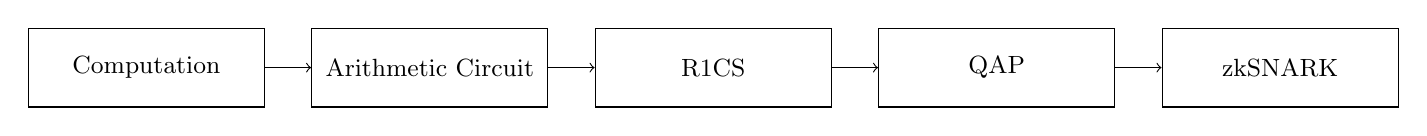
\begin{tikzpicture}[
    flow/.style={rectangle, minimum width=3cm, minimum height=1cm, text centered, draw=black,font=\small},
    scale=0.9
  ]
    \node[flow] (comp) at (0, 0) {Computation};
    \node[flow] (alg) at (4, 0) {Arithmetic Circuit};
    \node[flow] (r1cs) at (8, 0) {R1CS};
    \node[flow] (qap) at (12, 0) {QAP};
    \node[flow] (zk) at (16, 0) {zkSNARK};

    \draw[->] (comp) -- (alg);
    \draw[->] (alg) -- (r1cs);
    \draw[->] (r1cs) -- (qap);
    \draw[->] (qap) -- (zk);


  \end{tikzpicture}
  \caption{Steps of zk-SNARK}
  \label{fig:zkp:zksnark_flow}
\end{figure}

\subsubsection{Arithmetic circuits}
\label{zkp:snarks:circuits}

An arithmetic circuit $C$ over a finite field $\F$ is a circuit that contains
only addition and multiplication gates. It takes inputs that are elements in $\F$ and its gates output elements in $\F$~\cite{184425, zcash}.

Any program  can be reduced to  an arithmetic circuit~\cite{pankova_succinct_2013, 10.1007/978-3-642-40084-1_6} and normally the circuit is associated to the function it computes; the outsource function the Prover works upon.

Given a circuit evaluation, the task of the Prover is to convince the Verifier that there exist valuations of intermediate gates such that the circuit indeed produces such an output with such an input~\cite{pankova_succinct_2013}.

\begin{figure}[ht!]
  \center
  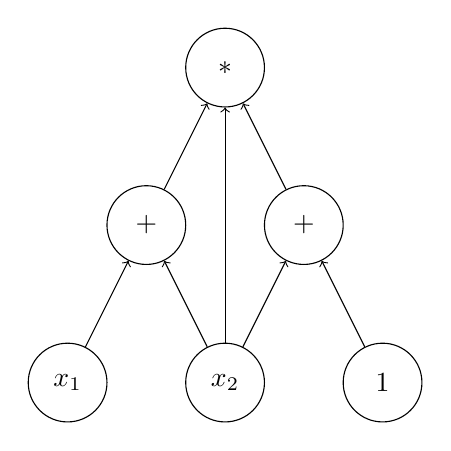
\begin{tikzpicture}[
        gate/.style={
        circle,
        minimum size=1cm,
        draw
      },
      node distance=2cm
    ]

    \node[gate] (x1) at (0, 0) {$x_1$};
    \node[gate] (x2) at (2, 0) {$x_2$};
    \node[gate] (1) at (4, 0) {$1$};

    \node[gate] (p1) at (1, 2) {$+$};
    \node[gate] (p2) at (3, 2) {$+$};

    \node[gate] (m1) at (2, 4) {$*$};

    \draw[->] (x1) -- (p1);
    \draw[->] (x2) -- (p1);
    \draw[->] (x2) -- (p2);
    \draw[->] (x2) -- (m1);

    \draw[->] (1) -- (p2);

    \draw[->] (p1) -- (m1);
    \draw[->] (p2) -- (m1);

  \end{tikzpicture}
  \caption{A simple arithmetic circuit}
  \label{fig:zkp:circuit}
\end{figure}

\subsubsection{Quadratic Arithmetic Program (QAP)}
\label{zkp:snarks:qap}

Geranno et. al~\cite{ggpr} showed how to encode efficiently computation as quadratic programs called Quadratic Arithmetic Programs (QSP), so as to obtain zk-SNARKs. A Quadratic Span Program consists of a set of polynomials and the task is to find a linear combination of those that is a multiple of another given polynomial.

\note{Implementations of zksnark (pinnochio, Hawk, Zcash etc)}
